%%%%%%%%%%%%%%%%%%%% book.tex %%%%%%%%%%%%%%%%%%%%%%%%%%%%%
%
% sample root file for the chapters of your "monograph"
%
% Use this file as a template for your own input.
%
%%%%%%%%%%%%%%%% Springer-Verlag %%%%%%%%%%%%%%%%%%%%%%%%%%


% RECOMMENDED %%%%%%%%%%%%%%%%%%%%%%%%%%%%%%%%%%%%%%%%%%%%%%%%%%%
\documentclass[envcountsame,envcountchap]{svmono}

% choose options for [] as required from the list
% in the Reference Guide, Sect. 2.2

\usepackage{makeidx}         % allows index generation
\usepackage{graphicx}        % standard LaTeX graphics tool
                             % when including figure files
\usepackage{multicol}        % used for the two-column index
\usepackage[bottom]{footmisc}% places footnotes at page bottom
\usepackage[utf8]{inputenc}
\usepackage[T1]{fontenc}
\usepackage{color}
\usepackage{listings}
\usepackage{float}

% etc.
% see the list of further useful packages
% in the Reference Guide, Sects. 2.3, 3.1-3.3

\makeindex             % used for the subject index
                       % please use the style svind.ist with
                       % your makeindex program


\floatstyle{ruled}
\newfloat{f_exemplo}{!ht}{lop}
\floatname{f_exemplo}{Exemplo}

%%%%%%%%%%%%%%%%%%%%%%%%%%%%%%%%%%%%%%%%%%%%%%%%%%%%%%%%%%%%%%%%%%%%%

\begin{document}

\author{João Filipe Meneses Henriques\\João Nuno Santos de Gusmão Guedes}
\title{Turn 12\\
{\small FEUP-PLOG, Turma 3MIEIC05, Grupo 17}}
\subtitle{-- Monograph --}
\maketitle

\frontmatter%%%%%%%%%%%%%%%%%%%%%%%%%%%%%%%%%%%%%%%%%%%%%%%%%%%%%%

%
%%%%%%%%%%%%%%%%%%%%%%% dedic.tex %%%%%%%%%%%%%%%%%%%%%%%%%%%%%%%%%
%
% sample dedication
%
% Use this file as a template for your own input.
%
%%%%%%%%%%%%%%%%%%%%%%%% Springer-Verlag %%%%%%%%%%%%%%%%%%%%%%%%%%

\thispagestyle{empty}
\vspace*{3.5cm}
\begin{flushright}

% write your text here
{\large Your dedication goes here}

\end{flushright}




%%%%%%%%%%%%%%%%%%%%%%% pref.tex %%%%%%%%%%%%%%%%%%%%%%%%%%%%%%%%%%%%%
%
% sample preface
%
% Use this file as a template for your own input.
%
%%%%%%%%%%%%%%%%%%%%%%%% Springer-Verlag %%%%%%%%%%%%%%%%%%%%%%%%%%

\preface

%% Please write your preface here
Here come the golden words


%% Please "sign" your preface
\vspace{1cm}
\begin{flushright}\noindent
place(s),\hfill {\it First name  Surname}\\
month year\hfill {\it First name  Surname}\\
\end{flushright}




\tableofcontents


\mainmatter%%%%%%%%%%%%%%%%%%%%%%%%%%%%%%%%%%%%%%%%%%%%%%%%%%%%%%%

%%%%%%%%%%%%%%%%%%%%% chapter.tex %%%%%%%%%%%%%%%%%%%%%%%%%%%%%%%%%
%
% sample chapter
%
% Use this file as a template for your own input.
%
%%%%%%%%%%%%%%%%%%%%%%%% Springer-Verlag %%%%%%%%%%%%%%%%%%%%%%%%%%

\chapter{Resumo}
\label{abstract} % Always give a unique label
% use \chaptermark{}
% to alter or adjust the chapter heading in the running head

Este artigo foi elaborado no contexto do curso de Programação em Lógica, e incide sobre a programação em lógica com restrições. 
A programação em lógica com restrições permite restringir problemas por domínio de soluções e por condições que devem ser cumpridas. 

Com o objectivo de avaliar a viabilidade da programação com restrições para resolver problemas de lógica de complexidade relevante, foram desenvolvidos algoritmos de resolução e de geração de novas soluções para dimensões variáveis do jogo Turn 12.
Para o efeito fez-se recurso à biblioteca de restrições para o cojunto dos domínios finitos clp(FD) do SICStus Prolog.

O método utilizado compreende a rotação dos dígitos de cada face, sendo o domínio o conjunto de rotações possíveis. A combinação das faces é feita iterativamente e não simultâneamente, por forma a optimizar os recursos.

Obtiveram-se resultados em tempo útil para solucionar o problema original e para um número de digitos não superior a 60, o que permitiu concluir que a metodologia utilizada é adequada para a resolução de problemas do género.

%%%%%%%%%%%%%%%%%%%%% introduction.tex %%%%%%%%%%%%%%%%%%%%%%%%%%%%%%%%%
%
% Introduction chapter
%
%%%%%%%%%%%%%%%%%%%%%%%% Springer-Verlag %%%%%%%%%%%%%%%%%%%%%%%%%%

\chapter{Introducão}
\label{introduction} % Always give a unique label
% use \chaptermark{}
% to alter or adjust the chapter heading in the running head

Programação em lógica com restrições é uma junção de dois paradigmas: solução de restrições e programação em lógica. Esta combinação permite uma concepção mais expressiva e flexível — e em alguns casos mais eficiente - de problemas lógicos.

\section{Motivação}
\label{sec:1}
% Always give a unique label
% and use \ref{<label>} for cross-references
% and \cite{<label>} for bibliographic references
% use \sectionmark{}
% to alter or adjust the section heading in the running head
A motivação deste trabalho incidiu na compreensão de um paradigma de programação que já nos é familiar, envolvendo uma nova componente de restrições; resolver problemas lógicos com restrições de uma forma geral, tendo a possibilidade de os refinar e otimizar para uma solução particular.

\section{Objectivos}
\label{sec:2}
Resolver a versão original do jogo Turn12 recorrendo a restrições; gerar cubos com um número de dígitos variável, e avaliar se estes têm solução ou não segundo as restrições definidas.

\section{Descrição do problema}
\label{sec:3}
O problema centra-se num cubo em que cada face contém dígitos numerados de 3 a 9, aleatoriamente. Na junção das arestas de cada face, a soma dos dois dígitos que se encontram deverá ser igual a 12.

A solução original (Fig. 2.1) com 24 dígitos por face é única.

A resolução que apresentamos contempla dígitos ilimitados, e uma vez que não existe qualquer padrão associado à sequência de dígitos no problema original, estes são gerados aleatóriamente e não é garantida a unicidade de solução.

No entanto, para valores demasiado elevados (superiores a 60 por face), as limitações de computação começaram-se a sentir e encontrar uma solução em tempo útil não foi possível, por limitações de Hardware.

%Figura cubo
\begin{figure}[h!]
\begin{center}
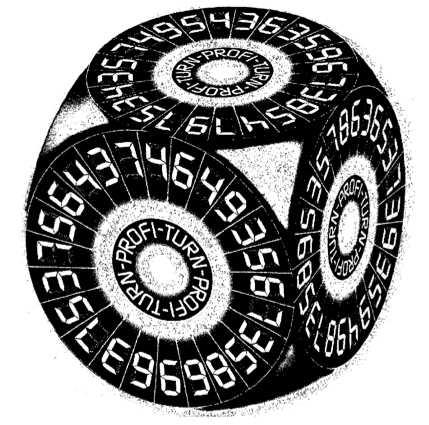
\includegraphics[scale=0.4]{turn12.png}
\caption{Problema original}
\label{fig:1}
\end{center}
\end{figure}

%

%%%%%%%%%%%%%%%%%%%%% restrictions.tex %%%%%%%%%%%%%%%%%%%%%%%%%%%%%%
%
% sample chapter
%
% Use this file as a template for your own input.
%
%%%%%%%%%%%%%%%%%%%%%%%% Springer-Verlag %%%%%%%%%%%%%%%%%%%%%%%%%%

\section{Ficheiros de Dados}
\label{data:1}

Os ficheiros de dados são simples ficheiros de texto (\textit{.txt}), que em cada linha têm os dígitos de cada face.
As faces encontram-se pela seguinte ordem: Topo, Baixo, Frente, Trás, Esquerda e por fim Direita.

De seguida encontra-se um exemplo deste ficheiro com os valores do problema original:

\begin{f_exemplo}[H]
\begin{verbatim}

356735869637537564374649
343574954363596738547975
353748635975458485676439
349576573795398457964379
357863653739359498735895
348765738453874583769785
\end{verbatim}
\caption{Problema original do turn12, com 24 dígitos por face:}
\end{f_exemplo}



\section{Variáveis de Decisão}
\label{restr:1}

As variáveis de decisão usadas na solução foram as rotações que podiam ser feitas em cada face do cubo.\\
Estas rotações têm um domínio compreendido entre 1 e o número de dígitos de cada face.

\section{Restrições}
\label{restr:2}

Independentemente do número de dígitos em cada face, verificou-se que as restrições seriam sempre as mesmas: a soma dos dígitos dos cantos onde cada face se toca, teria de ser 12.\\

De forma a fazer a sua implementação, foi utilizado no \textit{SICStus Prolog} a biblioteca de restrições para o conjunto dos domínios finitos \textit{clp(FD)}, onde foram definidas variáveis que seriam preenchidas com os valores dos cantos tendo em conta a rotação aplicada sobre cada face, e restringidas de forma que a soma onde todas se tocam ser obrigatoriamente 12.

\section{Função de Avaliação}
\label{restr:3}

A predicados de avaliação chamam-se \textit{turn12}. Existem três implementados (com o mesmo nome) na solução, mas o principal aceita como parâmetros de entrada as 6 faces do cubo, que deverão ser cada um uma lista numérica de dígitos. Se for encontrada uma solução, são definidas como parâmetros de saída as rotações respectivas a cada face. São também definidos e agrupados 4 a 4 os valores da solução. Este predicado tem como objectivo apenas retornar a primeira solução encontrada.\\
Outro predicado, com o mesmo nome, tem como parâmetro de entrada, a localização do ficheiro com a informação de cada face, e só termina ate imprimir todas as soluções que um problema pode ter.
Por fim, existe ainda uma última função que não aceita qualquer parâmetro, e que chama o predicado anteriormente descrito, com um ficheiro numa localização predefinida.


\section{Estratégia de Pesquisa}
\label{rest:4}

A estratégia de pesquisa tem como base começar por rodar cada face até encontrar uma solução.
De forma a optimizar a resolução do problema, o algoritmo começa apenas com duas faces, e tenta encontrar através do predicado de etiquetagem \textit{labeling}, uma rotação para cada que consiga somar o valor 12 onde ambas se tocam.
Quando encontrada, é passada para outra face do cubo, e com recurso a outro predicado de etiquetagem é tentado encontrar uma rotação para esta última que consiga satisfazer as mesmas restrições para os cantos em comum com as duas faces anteriores. É seguida sempre a mesma estratégia para as restantes faces, fazendo que a complexidade algorítmica seja sempre o mais inferior possível.
A razão para a utilização de vários predicados de etiquetagem deve-se ao facto de ser utilizado um predicado auxiliar (\textit{shifted\_face}) que preenche as variáveis utilizadas para testar as restrições com base na rotação correspondente, e tendo-se verificado que quando utilizado um único predicado para o mesmo efeito, o \textit{shifted\_face} era chamado desnecessariamente, mesmo para as faces em que a rotação se mantinha igual e que não tinham originado a falha.
Após isolados, o predicado só passou a ser chamado para a face do respectivo labeling, e evitando um varrimento contínuo e dispendioso nas várias listas de dígitos de cada face.

%


%\appendix
%\include{appendix}

\backmatter%%%%%%%%%%%%%%%%%%%%%%%%%%%%%%%%%%%%%%%%%%%%%%%%%%%%%%%

\chapter*{Solutions}
\addcontentsline{toc}{chapter}{Solutions}
\markboth{Solutions}{Solutions}

\section*{Problems of Chapter~\ref{intro}}

\begin{sol}{prob1}
The solution is revealed here.
\end{sol}


\begin{sol}{prob2}
\textbf{Problem Heading}\\
(a) The solution of first part is revealed here.\\
(b) The solution of second part is revealed here.
\end{sol}


%%%%%%%%%%%%%%%%%%%%%%%% referenc.tex %%%%%%%%%%%%%%%%%%%%%%%%%%%%%%
% sample references
% "computer science"
%
% Use this file as a template for your own input.
%
%%%%%%%%%%%%%%%%%%%%%%%% Springer-Verlag %%%%%%%%%%%%%%%%%%%%%%%%%%

%
% BibTeX users please use
% \bibliographystyle{}
% \bibliography{}
%
% Non-BibTeX users please use
\begin{thebibliography}{99.}
%
% and use \bibitem to create references.
%
% Use the following syntax and markup for your references
%
% Monographs
\bibitem{monograph} Kajan E (2002)
Information technology encyclopedia and acronyms. Springer, Berlin
Heidelberg New York

% Contributed Works
\bibitem{contribution} Broy M (2002) Software engineering -- From
auxiliary to key technologies. In: Broy M, Denert E (eds)
Software Pioneers. Springer, Berlin Heidelberg New York

% Journal
\bibitem{journal} Che M, Grellmann W, Seidler S (1997)
Appl Polym Sci 64:1079--1090

% Theses
\bibitem{thesis} Ross DW (1977) Lysosomes and storage diseases. MA
Thesis, Columbia University, New York

\end{thebibliography}

\printindex

%%%%%%%%%%%%%%%%%%%%%%%%%%%%%%%%%%%%%%%%%%%%%%%%%%%%%%%%%%%%%%%%%%%%%%

\end{document}





